\section{PageRank Beyond the Web}

\begin{bigidea}
The PageRank vector is the dominant eigenvector of the adjacency matrix of a directed graph and it ranks the importance of each vertex in the graph.
\end{bigidea}

\begin{definition}
Consider a directed graph $G$ with $N$ vertices (see \href{https://en.wikipedia.org/wiki/Directed_graph}{Wikipedia: Directed graph}). The {\bf adjacency matrix} is the $N \times N$ matrix $A = [a_{i,j}]$ where
$$
a_{i,j} = \left\{ \begin{array}{cc} 1 & \text{ if there is an edge to vertex $i$ from vertex $j$} \\ 0 & \text{ if not } \end{array} \right.
$$
Suppose the vertices of $G$ represent a collection webpages and the edges represent links from one webpage to another. (We only count one link maximum from one webpage to another and no links from a webpage to itself.) The {\bf stochastic matrix} \cite[p.134]{KN} of $G$ represents the process of clicking a random link on a webpage and is given by $P = [p_{i,j}]$ where
$$
p_{i,j} = \frac{a_{i,j}}{\text{total $\#$ of links from webpage $j$}}
$$
The entry $p_{i,j}$ is the probability of clicking to webpage $i$ from webpage $j$.
\end{definition}

\begin{example}
Consider the directed graph
\begin{center}
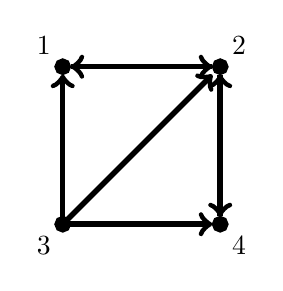
\begin{tikzpicture}[scale=2.0,line width=2pt]
\filldraw (0,0) circle (1pt); \filldraw (0,1) circle (1pt);
\filldraw (1,1) circle (1pt); \filldraw (1,0) circle (1pt);
\draw (0,1) node[anchor=south east] {1};
\draw (1,1) node[anchor=south west] {2};
\draw (1,0) node[anchor=north west] {4};
\draw (0,0) node[anchor=north east] {3};
\draw [->] (0,0) to (0,0.95);
\draw [->] (0,0) to (0.95,0);
\draw [->] (0,0) to (0.95,0.95);
\draw [->] (1,0.95) to (1,0.05);
\draw [->] (1,0.05) to (1,0.95);
\draw [->] (0.05,1) to (0.95,1);
\draw [->] (0.95,1) to (0.05,1);
\end{tikzpicture}
\end{center}
Construct the adjacency matrix $A$ and the stochastic matrix $P$
$$
A = \begin{bmatrix} 0 & 1 & 1 & 0 \\ 1 & 0 & 1 & 1 \\ 0 & 0 & 0 & 0 \\ 0 & 1 & 1 & 0 \end{bmatrix}
\hspace{10mm}
P = \begin{bmatrix} 0 & 1/2 & 1/3 & 0 \\ 1 & 0 & 1/3 & 1 \\ 0 & 0 & 0 & 0 \\ 0 & 1/2 & 1/3 & 0 \end{bmatrix}
$$
\end{example}

\begin{definition}
The {\bf Google matrix} of a directed graph $G$ is
$$
\alpha P + (1 - \alpha) \bs{v} \bs{e}^T
$$
where $P$ is the stochastic matrix of $G$, $0 < \alpha < 1$ is the {\bf teleportation parameter} \cite[p.322]{DG}, $\bs{v}$ is the {\bf teleportation distribution vector} and $\bs{e}^T = \begin{bmatrix} 1 & \cdots & 1 \end{bmatrix}$ is a vector of 1s. Note $\bs{v} \bs{e}^T$ is the matrix with vector $\bs{v}$ in every column.
\end{definition}

\begin{note}
The teleportation vector $\bs{v}$ has entries between 0 and 1 and the entries sum to 1. In other words, it is a stochastic vector. The vector $\bs{v}$ is usually chosen to be $\bs{v} = (1/N)\bs{e}$ where $N$ is the number of vertices in the graph. The stochastic matrix $\bs{v} \bs{e}^T$ then represents the process of transitioning to a random webpage with uniform probability. The Google matrix is a stochastic matrix which represents the process: at each step, do either:
\begin{itemize}
\item probability $\alpha$: click a random link on the webpage to visit another webapge
\item probability $1 - \alpha$: teleport to any webpage according to the distribution $\bs{v}$
\end{itemize}
The teleportation parameter $\alpha$ is usually chosen to be $\alpha = 0.85$.
\end{note}

\begin{proposition}
Let $G$ be a directed graph and let $P$ be the stochastic matrix for $G$. Choose parameters $0 < \alpha < 0$ and $\bs{v}$. There exists a unique steady state vector $\bs{x}$ (with entries between 0 and 1 and the entries sum to 1) such that
$$
\left( \alpha P + (1 - \alpha) \bs{v} \bs{e}^T \right) \bs{x} = \bs{x}
$$
The vector $\bs{x}$ is called the {\bf PageRank} vector and the entry $x_i$ is the PageRank of the webpage at vertex $i$. The Google search result lists the webpages in order of their PageRank.
\end{proposition}

\begin{note}
A directed graph $G$ represents a collection of webpages that contain the words in a Google search. The PageRank vector ranks the importance of the webpages for the search. There are usually hundreds of millions webpages in the graph therefore the Google matrix is HUGE! But the founders of Google showed that the power iteration algorithm converges well enough after about 50 iterations to find the webpages with the top PageRank.
\end{note}

\begin{example}
Find the Google matrix for the directed graph in the example above for $\alpha = 0.85$ and $\bs{v} = (1/N) \bs{e}$. Compute
\begin{align*}
\alpha P + (1 - \alpha) \bs{v} \bs{e}^T &=
0.85 \begin{bmatrix} 0 & 1/2 & 1/3 & 0 \\ 1 & 0 & 1/3 & 1 \\ 0 & 0 & 0 & 0 \\ 0 & 1/2 & 1/3 & 0 \end{bmatrix}
+
\frac{0.15}{4}
\begin{bmatrix} 1 & 1 & 1 & 1 \\ 1 & 1 & 1 & 1 \\ 1 & 1 & 1 & 1 \\ 1 & 1 & 1 & 1 \end{bmatrix} \\
&=
\begin{bmatrix}
0.0375 & 0.4625 & 0.3208 & 0.0375 \\
0.8875 & 0.0375 & 0.3208 & 0.8875 \\
0.0375 & 0.0375 & 0.0375 & 0.0375 \\
0.0375 & 0.4625 & 0.3208 & 0.0375
\end{bmatrix}
\end{align*}
Compute 50 iterations of the power method to approximate the PageRank vector
$$
\bs{x} \approx \begin{bmatrix} 0.2472 \\ 0.4681 \\ 0.0375 \\ 0.2472 \end{bmatrix}
$$
Clearly, vertex 2 is the most important in the graph.
\end{example}
